\documentclass[journal,12pt,twocolumn]{IEEEtran}

\usepackage{setspace}
\usepackage{gensymb}

\singlespacing


\usepackage[cmex10]{amsmath}

\usepackage{amsthm}

\usepackage{mathrsfs}
\usepackage{txfonts}
\usepackage{stfloats}
\usepackage{bm}
\usepackage{cite}
\usepackage{cases}
\usepackage{subfig}

\usepackage{longtable}
\usepackage{multirow}

\usepackage{enumitem}
\usepackage{mathtools}
\usepackage{steinmetz}
\usepackage{tikz}
\usepackage{circuitikz}
\usepackage{verbatim}
\usepackage{tfrupee}
\usepackage[breaklinks=true]{hyperref}
\usepackage{graphicx}
\usepackage{tkz-euclide}
\usepackage{float}

\usetikzlibrary{calc,math}
\usepackage{listings}
\usepackage{color} %%
\usepackage{array} %%
\usepackage{longtable} %%
\usepackage{calc} %%
\usepackage{multirow} %%
\usepackage{hhline} %%
\usepackage{ifthen} %%
\usepackage{lscape}
\usepackage{multicol}
\usepackage{chngcntr}

\DeclareMathOperator*{\Res}{Res}

\renewcommand\thesection{\arabic{section}}
\renewcommand\thesubsection{\thesection.\arabic{subsection}}
\renewcommand\thesubsubsection{\thesubsection.\arabic{subsubsection}}

\renewcommand\thesectiondis{\arabic{section}}
\renewcommand\thesubsectiondis{\thesectiondis.\arabic{subsection}}
\renewcommand\thesubsubsectiondis{\thesubsectiondis.\arabic{subsubsection}}


\hyphenation{op-tical net-works semi-conduc-tor}
\def\inputGnumericTable{} %%

\lstset{
%language=C,
frame=single,
breaklines=true,
columns=fullflexible
}
\begin{document}


\newtheorem{theorem}{Theorem}[section]
\newtheorem{problem}{Problem}
\newtheorem{proposition}{Proposition}[section]
\newtheorem{lemma}{Lemma}[section]
\newtheorem{corollary}[theorem]{Corollary}
\newtheorem{example}{Example}[section]
\newtheorem{definition}[problem]{Definition}

\newcommand{\BEQA}{\begin{eqnarray}}
\newcommand{\EEQA}{\end{eqnarray}}
\newcommand{\define}{\stackrel{\triangle}{=}}
\bibliographystyle{IEEEtran}
\providecommand{\mbf}{\mathbf}
\providecommand{\pr}[1]{\ensuremath{\Pr\left(#1\right)}}
\providecommand{\qfunc}[1]{\ensuremath{Q\left(#1\right)}}
\providecommand{\sbrak}[1]{\ensuremath{{}\left[#1\right]}}
\providecommand{\lsbrak}[1]{\ensuremath{{}\left[#1\right.}}
\providecommand{\rsbrak}[1]{\ensuremath{{}\left.#1\right]}}
\providecommand{\brak}[1]{\ensuremath{\left(#1\right)}}
\providecommand{\lbrak}[1]{\ensuremath{\left(#1\right.}}
\providecommand{\rbrak}[1]{\ensuremath{\left.#1\right)}}
\providecommand{\cbrak}[1]{\ensuremath{\left\{#1\right\}}}
\providecommand{\lcbrak}[1]{\ensuremath{\left\{#1\right.}}
\providecommand{\rcbrak}[1]{\ensuremath{\left.#1\right\}}}
\theoremstyle{remark}
\newtheorem{rem}{Remark}
\newcommand{\sgn}{\mathop{\mathrm{sgn}}}
\providecommand{\abs}[1]{\left\vert#1\right\vert}
\providecommand{\res}[1]{\Res\displaylimits_{#1}}
\providecommand{\norm}[1]{\left\lVert#1\right\rVert}
%\providecommand{\norm}[1]{\lVert#1\rVert}
\providecommand{\mtx}[1]{\mathbf{#1}}
\providecommand{\mean}[1]{E\left[ #1 \right]}
\providecommand{\fourier}{\overset{\mathcal{F}}{ \rightleftharpoons}}
%\providecommand{\hilbert}{\overset{\mathcal{H}}{ \rightleftharpoons}}
\providecommand{\system}{\overset{\mathcal{H}}{ \longleftrightarrow}}
%\newcommand{\solution}[2]{\textbf{Solution:}{#1}}
\newcommand{\solution}{\noindent \textbf{Solution: }}
\newcommand{\cosec}{\,\text{cosec}\,}
\providecommand{\dec}[2]{\ensuremath{\overset{#1}{\underset{#2}{\gtrless}}}}
\newcommand{\myvec}[1]{\ensuremath{\begin{pmatrix}#1\end{pmatrix}}}
\newcommand{\mydet}[1]{\ensuremath{\begin{vmatrix}#1\end{vmatrix}}}
\numberwithin{equation}{subsection}
\makeatletter
\@addtoreset{figure}{problem}
\makeatother
\let\StandardTheFigure\thefigure
\let\vec\mathbf
\renewcommand{\thefigure}{\theproblem}
\def\putbox#1#2#3{\makebox[0in][l]{\makebox[#1][l]{}\raisebox{\baselineskip}[0in][0in]{\raisebox{#2}[0in][0in]{#3}}}}
\def\rightbox#1{\makebox[0in][r]{#1}}
\def\centbox#1{\makebox[0in]{#1}}
\def\topbox#1{\raisebox{-\baselineskip}[0in][0in]{#1}}
\def\midbox#1{\raisebox{-0.5\baselineskip}[0in][0in]{#1}}
\vspace{3cm}
\title{Assignment No.1} 
\author{Suyog Tangade\\MD/2020/710} 
\maketitle
\newpage
\bigskip
\renewcommand{\thefigure}{\theenumi}
\renewcommand{\thetable}{\theenumi}
Download all python codes from
\begin{lstlisting}
https://github.com/suyogtangade/AI.gi
\end{lstlisting}
%
and latex-tikz codes from
%
\begin{lstlisting}
https://github.com/suyogtangade/AI.git
\end{lstlisting}
%
\section{Question No.16(b) (cbse/2006/set-2)}

Find the co-ordinates of the point equidistant from three given points $\vec{A}\myvec{5\\3}$, $\vec{B}\myvec{5\\-5}$ and $\vec{C}\myvec{1\\-5}$ 
\solution

Let the point equidistant from $\Vec{A}$ \& $\Vec{B}$ \& $\Vec{C}$ be 
\begin{align}
    \Vec{P}=\myvec{x\\y}
\end{align}
From the given information 
\begin{align}\label{eq:1}
    \norm{\Vec{P}-\vec{A}}^2 &= \norm{\vec{P}-\vec{B}}^2 = \norm{\vec{P}-\vec{C}}^2\\
\therefore
    \norm{\Vec{P}-\vec{A}}^2 &= \norm{\vec{P}-\vec{B}}^2
\end{align}

\begin{equation} \label{eq:2}
\boxed{(\vec{P}-\vec{A})^{\top}(\vec{P}-\vec{A})=(\vec{P}-\vec{B})^{\top}(\vec{P}-\vec{B})}
\end{equation}
\begin{align}
 (\vec{P}-\vec{A})^{\top}(\vec{P}-\vec{A})=\vec{P}^{\top} \vec{P}-\vec{P}^{\top} \vec{A}-\vec{A}^{\top} \vec{P}+\vec{A}^{\top} \vec{A}
\\
(\vec{P}-\vec{B})^{\top}(\vec{P}-\vec{B})=\vec{P}^{\top} \vec{P}-\vec{P}^{\top} \vec{B}-\vec{B}^{\top} \vec{P}+\vec{B}^{\top} \vec{B}   
\end{align}
Consider the expressions 
\begin{align}
\vec{P}^{\top} \vec{P}=\norm{\vec{P}}^2\\
\vec{P}^{\top} \vec{A}=\vec{A}^{\top} \vec{P}
\end{align}
Final expression of \eqref{eq:2} can be written as
\begin{align}
\boxed{\norm{\vec{P}}^2-2 \vec{A}^{\top} \vec{P}+\vec{A}^{\top} \vec{A}=\norm{\vec{P}}^2-2 \vec{B}^{\top} \vec{P}+\vec{B}^{\top} \vec{B}}\\
\implies-2 \vec{A}^{\top} \vec{P}+2 \vec{B}^{\top} \vec{P}= \vec{B}^{\top} \vec{B}-\vec{A}^{\top} \vec{A}\\
\implies 2 \vec{P}(\vec{A}^{\top}-\vec{B}^{\top})= \vec{A}^{\top} \vec{A}-\vec{B}^{\top} \vec{B}
\end{align}
\begin{equation} \label{eq:3}
2 \vec{P}(\vec{A}^{\top}-\vec{B}^{\top})=\norm{\vec{A}}^2-\norm{\vec{B}}^2
\end{equation}
\vec{P} lies on the y-axis
\begin{equation}
    \boxed{\vec{P}&= y\myvec{0\\1}&= y \vec{e_2}}
\end{equation}
Now substitute this in \eqref{eq:3}
\begin{align}
2\vec{ye_2}(\vec{A}^{\top}-\vec{B}^{\top})&=\norm{\vec{A}}^2-\norm{\vec{B}}^2\\
\boxed{\vec{y} = \frac{\norm{\vec{A}}^2 - \norm{\vec{B}}^2}{2\vec{e_2}(\vec{A}^{\top} - \vec{B}^{\top})}}\\
\vec{2e_2}(\vec{A}^{\top}-\vec{B}^{\top})&=2\myvec{0\\1}\myvec{0\ 8}=16\\
\implies
\vec{y}&=\myvec{\dfrac{-16}{16}}\\
 \boxed{\therefore \vec{y} =-1}
\end{align}
From \eqref{eq:1} we can write
\begin{align}
   \norm{\Vec{P}-\vec{B}}^2 &= \norm{\vec{P}-\vec{C}}^2 
\end{align}

\begin{equation} \label{eq:4}
2 \vec{P}(\vec{B}^{\top}-\vec{C}^{\top})=\norm{\vec{B}}^2-\norm{\vec{C}}^2
\end{equation}
\vec{P} lies on the x-axis
\begin{equation}
     \boxed{\vec{P}&= x\myvec{1\\0}&= x \vec{e_2}}
\end{equation}
Now substitute this in \eqref{eq:4}
\begin{align}
2\vec{xe_2}(\vec{B}^{\top}-\vec{C}^{\top})&=\norm{\vec{B}}^2-\norm{\vec{C}}^2\\
\boxed{\vec{x} = \frac{\norm{\vec{B}}^2 - \norm{\vec{C}}^2}{2\vec{e_2}(\vec{B}^{\top} - \vec{C}^{\top})}}\\
\vec{2e_2}(\vec{B}^{\top}-\vec{C}^{\top})&=2\myvec{1\\0}\myvec{4\ 0}=8\\
\implies
\vec{x}&=\myvec{\dfrac{24}{8}}\\
 \boxed{\therefore \vec{x} =3}
\end{align}\\
The coordinate  point  equidistance from three points is
\numberwithin{figure}{section}
\begin{figure}
    \centering
    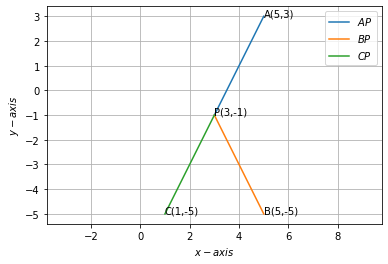
\includegraphics{Figure.png}
    \caption{Graphical Solution}
    \label{fig:my_label}
\end{figure}\\
\begin{align}
    \vec{P}=\myvec{3\\-1}.
\end{align}\\
\end{document}
